%%
%% Meta: TI nSpire Einführung
%%       Ziel: Damit die Grundoperationen damit durchgeführt werden können.
%%             Damit man sich an den Rechner gewöhnt.
%%

%% Philipp G Freimann Juli 2019 für die BBW
%% Phi BBW-Vorlage für Arbeitsblätter (LaTeX)
%% 2019 - 08 - 18

%% %% %% %%
\documentclass[twoside,12pt,a4paper]{article}%%
\usepackage[paper=a4paper,margin=17mm]{geometry}%%


%% Zentralisiert
%%\usepackage{german} %% Macht Probleme mit grafiken
\usepackage{mciteplus}

\usepackage[dvipsnames,table]{xcolor}

\usepackage{pgfplotstable}
\usepackage{tikz}
\usepackage{tkz-euclide} %% Grid

\usepackage{amsthm}
\usepackage{amsfonts} %% Zahlmengen Z, R, ...


%% THEOREMS?
\usepackage{tcolorbox}
\tcbuselibrary{theorems}
\tcbuselibrary{skins}


\usepackage{fancyhdr}
\usepackage{ngerman}
\usepackage[utf8]{inputenc}


%%\usepackage[dvips]{graphicx}

\usepackage{supertabular}
\usepackage{makeidx}  
\usepackage{ifthen} 

\usepackage{multirow}
\usepackage{listings}

%%\usepackage{color,fancyvrb,fancybox}
\usepackage{multicol}
\usepackage{lastpage}
%%\usepackage{listings}
\usepackage{pstricks}

%% bold typewriter font:
\usepackage[T1]{fontenc}
\usepackage{lmodern}

\usepackage{enumitem}
%\usepackage{enumerate}

\usepackage{float}

\usepackage{titlesec}
\usepackage{textcomp}

%% Kuchendiagramme
%%\usepackage{datapie}

%% für Aufgaben Hervorhebung
%%\usepackage[most]{tcolorbox}
%%\usepackage[standard,framed]{ntheorem}
\usepackage{framed}
\usepackage{mdframed}

%%%%%%%%%%%%%%%%%%%%
%%\usepackage[most]{tcolorbox}

\usepackage[tocindentauto]{tocstyle}

%% für accentset wedge:
\usepackage{accents}

%% Würfel
\usepackage{epsdice}

%% Einbinden von GeoGebra Bildchen:
\usetikzlibrary{shapes.geometric}
\usetikzlibrary{arrows}
\newcommand{\degre}{\ensuremath{^\circ}}

%% Hyperlinks
\usepackage{hyperref}

\hypersetup{
    colorlinks=true,
    linkcolor=blue,
    filecolor=magenta,      
    urlcolor=cyan,
    bookmarks=true,
}

%% bugtracker (part of pgfplots) should be loaded AFTER "hyperref"
%% See: https://texblog.net/hyperref/ AND https://tex.stackexchange.com/questions/16268/warning-with-footnotes-namehfootnote-xx-has-been-referenced-but-does-not-exi
\usepackage{pgfplots}
\pgfplotsset{width=10cm,compat=1.9}

%%\usepackage{fourier}  %% eg overarc (Bogenmaß)

%%%%%%%%%%%%%%%%% L A Y O U T  %%%%%%%%%%%%%%%%%%%%%%%%%%%%
%% 2020-12-27 ph. g. freimann @ bbw.ch
%%

\fancyhf{}%%

\pagestyle{fancy}%%

\renewcommand{\sectionmark}[1]{%%
  \markboth{\thesection{} \ #1}{}%%
}%%

\renewcommand{\subsectionmark}[1]{%%
  \markright{\thesubsection \ #1}%%
}%%

%% Achtung: chaptermark nur im BOOK-Style

\renewcommand{\footrulewidth}{0.4pt}

\parskip4pt
\parindent0pt

\topmargin-2.0cm
\textheight24.4cm

\renewcommand{\arraystretch}{1}%%


\newenvironment{bbwFillInTabular}{%%
%% BEGIN PART:
\renewcommand{\arraystretch}{2.1}
\begin{tabular}%%
}%% END PART:
{\end{tabular}
\renewcommand{\arraystretch}{1}%%
}%% END Environment bbwFillInTabular

%%%%%%%%%%%%%%%%%%%%%%%%%%%%%%%%%%%%%%%%%%%%%%%%%%%%%%%%%%
%%%%%%%%%%%%%%%%%% M A K R O S %%%%%%%%%%%%%%%%%%%%%%%%%%%
%%%%%%%%%%%%%%%%%%%%%%%%%%%%%%%%%%%%%%%%%%%%%%%%%%%%%%%%%%

%%%%%%%%%%%%%%%%%%%%%%%% g e n e r e l l e   M a k r o s %%%%%%%%%%%%%%%%%%%%%%%

%% Info vorab bei \newcommand
%% \newcommand{ - Kommandos können in den Parametern auch Leerzeilen
%%     enthalten
%% \newcommand*{ - Kommandos, also mit *, können jedoch in den
%%    Argumenten KEINE \par (sprich Leerzeilen} enthalten

%% 2019-07-26
%% phi@freimann.eu
%% Makros for BBW-Tex Documents
\usepackage{inputs/bbwColors}

%%%%%%%%%%%%%%%%%% I N C L U D E S   &   I N D E X  %%%%%
\graphicspath{{../img/}}
\graphicspath{{./img/}}

\newcommand*\bbwGraphicRaise[3]{\raisebox{#1}{\includegraphics[width=#2]{#3}}}%%
\newcommand*\bbwGraphic[2]{\bbwGraphicRaise{-5mm}{#1}{#2}}%%
\newcommand*\bbwCenterGraphicRaise[3]{\begin{center}\bbwGraphicRaise{#1}{#2}{#3}\end{center}}
\newcommand*\bbwCenterGraphic[2]{\bbwCenterGraphicRaise{-5mm}{#1}{#2}}%%


%% All in one Skript
\newif\ifisALLINONE
\isALLINONEfalse

%% Blended Learning
%% Insb. MatheNinja Links. Diese sind jedoch in einem anderen Kurs!
\newif\ifisBLENDED
\isBLENDEDfalse


%%%%%%%%% TRAINER Version vs. Schülerversion %%%%%%%%%%%%%
%% Bem. Kein *-Kommando, da die TRAINER-Blöcke auch leerzeilne (\par)
%% enthaltne können
\newcommand\TRAINER[1]{%%
{%%
\ifisTRAINER{\color{BlueGreen}{#1}}%%
\fi%%
}}%%  

\newcommand\TALS[1]{%
{%%
\ifisTALS{#1}%%
\fi%%
}}%

\newcommand\GESO[1]{%
{%%
\ifisGESO{#1}%%
\fi%%
}}%    

\newcommand\BLENDED[1]{%
{%%
\ifisBLENDED{#1}%%
\fi%%
}}%    

\newcommand{\noTRAINER}[1]{{\ifisTRAINER{}\else{#1}\fi}{}}%%



%%\makeatletter
%% Je nach Umgebung "environment" wird das mmPapier breiter oder
%% schmaler
%% bei itemize sollen 16.4 und bei definiton-Boxen 16.8 mm genommen
%% werden.


\usepackage{inputs/mmPapierbreiteSty}


%% Trainer "no" Dotfill
%% If no Trainer: Dotfill
\newcommand*{\TNDF}[1]{\TRAINER{#1}\noTRAINER{\dotfill{}}}%%

\newcommand*{\leserluft}{\vspace{2mm}}

%% Notiz felder 
%% Anwendung:
%% \noteField{10}  
%%  --> Notizfeld mit 10 Leerzeilen
\newcounter{DFCounter}


%%Häuschenpapier
\newcommand{\mmPapierZwei}[2]{\begin{tikzpicture}
%%  \draw[step=4mm,bbwMMFarbe,ultra thin]
%%  \draw[step=4mm,bbwMMFarbe,thick]
  \draw[step=4mm,bbwMMFarbe,line width=0.02mm]
  (0, 0) grid ({#2}, {#1});
\end{tikzpicture}}%%


%% millimeterPapier füllen bis Ende Seite
\newcommand{\mmPapierBisEndeSeite}{

\begin{tikzpicture}

\newdimen\spaceleftOnPage
\spaceleftOnPage=\dimexpr\textheight-\pagetotal-14pt\relax

\pgfmathsetmacro{\gridWidth}{\textwidth        - mod(\textwidth,      4mm)      }
\pgfmathsetmacro{\gridHeight}{\spaceleftOnPage - mod(\spaceleftOnPage,4mm) - 4mm}

\draw [step=4mm,bbwMMFarbe,line width=0.02mm] (0,0) grid (\gridWidth pt,\gridHeight pt);
\end{tikzpicture}%%
\newpage%%
}%% END Makro mmPapieBisEndeSeite


%% Standardbreite für Arbeitsblätter und das Theorieheft
%% Wird in bbwPruefung.sty überschrieben, da dort schmaler
\def\defaultTextBreite{17.6}
\def\unitCMWhatElse{cm}%% wird als Breitenangabe für den nächsten command verwendet

%% Verwendung: \bbwCenterGraphic{\defaultTextBreite}{«img url»}
\def\defaultTextBreiteCM{\defaultTextBreite\unitCMWhatElse}
\newcommand{\mmPapier}[1]{\mmPapierZwei{#1}{\defaultTextBreite}}


%% Notizen Berechungen auf Prüfungsblättern
\newcommand{\platzFuerBerechnungen}[1]{\noTRAINER{

Notizen / Berechnungen:

\mmPapier{#1}}}%% end platzFuerBerechnungen

\newcommand{\platzFuerBerechnungenBisEndeSeite}[1]{\noTRAINER{

Notizen / Berechnungen:

\mmPapierBisEndeSeite}}%% end platzFuerBerechnungen



\newcommand{\platzFuerBerechnungenOhneText}[1]{\noTRAINER{

\mmPapier{#1}}}

%% Die Abkürzung z.\,B. von «Zum Beispiel» hat einen verkleinerten Abstand.
\newcommand*\zB{%
z.\,B.
}

%%
%% Auf der Titelseite steht entweder GESO oder TALS.
%% Dies wird gleich mit der Fußnote angegeben.
%% Dieses Kommando sollte im Kommando «\untertitel» eingesetzt werden.
%%
\newcommand*\ausrichtungAufTitelseite{%
\ifisTALS{TALS\noTRAINER{\footnote{TALS «Technik, Architektur und Life Sciences
(Laboranten)»: Ausrichtung technisches Profil}}}%%
\fi%%
\ifisGESO{GESO\noTRAINER{\footnote{GESO: Ausrichtung \textbf{Ge}sundheit und \textbf{So}ziales}}}%%
\fi}%%

%%%%%%%%%%%%%%%%%%%%%% B B W - M a t h e   F a r b c o d e s  %%%%%%%%%%%%%%%%%%%%%%%%%%%%%%555

\newcommand{\rezeptFarbe}{rezeptFarbe}
\newcommand{\definitionFarbe}{definitionFarbe}
\newcommand{\gesetzFarbe}{gesetzFarbe}
\newcommand{\beispielFarbe}{beispielFarbe}
\newcommand{\bemerkungFarbe}{bemerkungFarbe}

%% Falls gewünscht übersteuren
%  \definecolor{xyz}{HTML}{eeff66}
%  \renewcommand{\beispielFarbe}{xyz}
%

%% Theorem-Styles
\newcommand\theoremlayoutdefinition[4]{\newtcbtheorem[number within=section]{#1}{#2}%
   {theorem style=plain,enhanced,colframe=#3!20!white,colback=#3!20!white,
     coltitle=#3!60!black,fonttitle=\upshape\bfseries,
     %%fontupper=\itshape,
    %%drop fuzzy shadow=blue!50!black!50!white,
    terminator sign={:},
    borderline north={0.5mm}{0pt}{#3}, borderline south={0.5mm}{0pt}{#3}
}{#4}}



%% Farben für rezept, definition und gesetz von Marthale übernommen.
%% Verwendung mit * unterbindet die Nummerierung \begin{gesetz*}{Blah}{xy} ...\end {gesetz*}
\theoremlayoutdefinition{rezept}{Rezept}{\rezeptFarbe}{R}
\theoremlayoutdefinition{definition}{Definition}{\definitionFarbe}{D}
\theoremlayoutdefinition{gesetz}{Gesetz}{\gesetzFarbe}{G}%% was green
\theoremlayoutdefinition{beispiel}{Beispiel}{\beispielFarbe}{B}
\theoremlayoutdefinition{bemerkung}{Bemerkung}{\bemerkungFarbe}{M}

%%
%% Force a blank page, when \newpage does not work
%%
\def\blankpage{%
	\clearpage%
	\null%
	\clearpage}%%

\newcommand{\Lueckentext}[1]{\,\,\noTRAINER{\dotfill}\TRAINER{#1}}


\newcommand{\LoesungsRaumCM}[2]{\,\,\noTRAINER{\underline{\hspace{#1}}}\TRAINER{#2}}

\newcommand{\LoesungsRaum}[1]{\LoesungsRaumCM{30mm}{#1}}
\newcommand{\LoesungsRaumKurz}[1]{\LoesungsRaumCM{15mm}{#1}}
\newcommand{\LoesungsRaumLang}[1]{\LoesungsRaumCM{45mm}{#1}}


%% TI nSpire
\def\tinspire{\texttt{TI-nSpire}}

%% TI 30 Pro Mathprint Button Images
\def\tiprobuttonbreite{10mm}
\def\nspirebuttonbreite{8.6mm}

%%\def\sec{\raisebox{-2mm}{\includegraphics[width=\buttonbreite{}]{img/tiprobuttonimages/2nd.png}}}
\newcommand{\tiprobutton}[1]{\raisebox{-2mm}{\mbox{\,\includegraphics[width=\tiprobuttonbreite{}]{img/tiprobuttonimages/#1.png}\,}}}

\newcommand{\nspirebutton}[1]{\raisebox{-2mm}{\mbox{\,\includegraphics[width=\nspirebuttonbreite{}]{img/nspirebuttonimages/#1.png}\,}}}

%% Counter  für Aufgaben
%% Bei jedem Part wird die Aufgabennummer zurückgesetz auf 1
\newcommand{\bbwPartID}{AA1}
\newcommand{\bbwAufgabenBlockID}{}
\newcounter{bbwAufgabenNummerCounter}[part]
\setcounter{bbwAufgabenNummerCounter}{1}
\newcommand{\bbwAufgabenNummer}{\arabic{bbwAufgabenNummerCounter}}
\newcommand{\nextBbwAufgabenNummer}{\stepcounter{bbwAufgabenNummerCounter}}
\newcommand{\aufgSubLabel}{{\color{blue}\bbwAufgabenNummer. \alph*)}}

%% Benutze außerhalb der bbwAufgabenblöcke folgendes Kommando, um an die
%% nächste Aufgabennummer zu kommen. Dies z. B. wenn ein längerer Text vor der Aufgabe steht,
%% der auch schon diese Bezeichnung erhalten sollte
\newcommand{\bbwActAufgabenNr}{{\color{blue}\bbwAufgabenNummer. {\small[\bbwAufgabenBlockID]}}}


\newenvironment{bbwAufgabenBlock}{%% Begin environment Part:

\bbwActAufgabenNr{}
%%{\color{blue}\bbwAufgabenNummer. {\small[\bbwAufgabenBlockID]}}
\begin{enumerate}[label=\aufgSubLabel]
}%% Ende der Präambel
{%% END Part:
\end{enumerate}
\nextBbwAufgabenNummer
}%% END environment bbwAufgabenBlock

%%%%%%%%%%%%%%%%%%%%%%%%%%%%

%% Weblinks und Mathe Ninja Links

\newcommand{\weblink}[2]{\href{#2}{#1}}

\newcommand{\olatBBWLogo}{
\includegraphics[width=15mm]{logos/traube.pdf}}%%
\newcommand{\externerLinkEPS}{
\includegraphics[width=15mm]{logos/extLink.pdf}}%%
\newcommand{\youtubeLogo}{\includegraphics[width=15mm]{logos/youtube.png}}%%


%%
%% #1: Text
%% #2: URL
%% #3: Aufgabennummern
%% #4: optional weitere Logos oder leer lassen {}
\newcommand{\externalLink}[4]{%%
\begin{tabular}{|lp{111mm}|}\hline%%
\multicolumn{2}{|p{172mm}|}{\cellcolor{aufgabenFarbe}#3}\\
\weblink{\raisebox{-5mm}{\externerLinkEPS{}}}{#2} {#4}  & \weblink{#1}{#2}\\\hline
\multicolumn{2}{|p{172mm}|}{\weblink{#2}{#2}}\\\hline
\end{tabular}%%
\vspace{1mm}
}%% END Command externalLink

%% #1: URL
%% #2: Text
\newcommand{\youtubeLink}[2]{%%
\externalLink{#2}{#1}{Youtube}{\raisebox{-5mm}{\youtubeLogo{}}}
}%%

%%
%% #1: Typ-Logo (eg. LOGO auf MatheNinja)
%% #2: Typ-Name (eg «Mathe Ninja»
%% #3: URL
%% #4: Aufgaben Name
\newcommand{\olatLink}[4]{%%
\begin{tabular}{|lp{111mm}|}\hline%%
\multicolumn{2}{|p{172mm}|}{\cellcolor{aufgabenFarbe}#4}\\
\weblink{\raisebox{-5mm}{\externerLinkEPS{}}}{#3} \weblink{\raisebox{-5mm}{\olatBBWLogo}}{#3} \weblink{#1}{#3}& \weblink{#2}{#3}\\\hline
\end{tabular}%%
\vspace{1mm}
}%% END Command olatLink


%\newcommand{\olatLOGOLink}[3]{%%
%\begin{tabular}{|lp{111mm}|}\hline%%
%\weblink{\raisebox{-5mm}{\olatBBWLogo{}}}{#2} & \weblink{#1}{#2}\\
%\multicolumn{2}{|p{172mm}|}{\cellcolor{aufgabenFarbe}#3}\\\hline
%\end{tabular}%%
%}%% END Command olatLOGOLink

%% Use:
%% \olatLinkArbeitsblatt{Kapitel/Arbeitsblattname «[ID]»}{«URL»}{Aufgabennummern}
\newcommand{\olatLinkArbeitsblatt}[3]{\olatLink{\raisebox{-6mm}{
\includegraphics[width=12mm]{logos/seite.pdf}}}{Arbeitsblatt: #1}{#2}{#3}}%%

%% #1: Text
%% #2: URL
\newcommand{\olatLinkPruefung}[2]{\olatLink{\raisebox{-6mm}{
\includegraphics[width=15mm]{logos/test.pdf}}}{Online Test}{#2}{#1}}%%


%%
%% use:
%% \matheNinjaLink{Beschreibung}{URL}
\newcommand{\matheNinjaLink}[2]{\olatLink{\raisebox{-6mm}{\includegraphics[width=17mm]{img/matheninja/matheninja.jpg}}}{Mathe Ninja!}{#2}{#1}}%%


%% Use
%% \olatLinkGESOKompendium{Kapitel}{Seite/Seiteff}{Aufgabe(n)}
\newcommand{\olatLinkGESOKompendium}[3]{%%
\GESO{%%
\olatLink{{\Huge K}}{Kompendium}{https://olat.bbw.ch/auth/RepositoryEntry/572162163/CourseNode/106029172671728}{Kapitel #1; Seite #2; Aufg. #3}%%
}%% END GESO
}%%


%% Use \olatLinkTALSStrukturaufgabenSPF{Kapitel}{Seite/Seiteff}{Aufgabe(n)}
\newcommand{\olatLinkTALSStrukturaufgabenSPF}[3]{%%
\TALS{%%
\olatLink{{\Huge S}}{Strukturaufgaben}{https://olat.bbw.ch/auth/RepositoryEntry/572162090/CourseNode/102901174299246}{Kapitel #1; Seite #2; Aufgaben #3}%%
}%% END GESO
}%%

%%\newcommand{\olatLinkTALtfSStrukturaufgabenGLF}[1]{\olatLOGOLink{Strukturaufgaben Grundlagenfach}{https://olat.bbw.ch/auth/RepositoryEntry/572162090/CourseNode/102901174291476}{#1}}


%%\newcommand{\matheNinjaLink}[2]{%%
%%\begin{tabular}{cc}%%
%% \raisebox{-1cm}{\includegraphics[height=2cm]{img/matheninja/turtle.png}}& \href{#2}{MatheNinja: #1}\\%%
%% \end{tabular}%%
%%}%% End Command  \matheNinjaLink



%% AadB = Aufgaben aus dem Buch
%% 1. Parameter: Seitenzahl
%% 2. Parameter: Aufgabennummern.
%% bsp  \TALSAadB{38-39}{101a-101c, 102 und 103}

%%\newcommand*{\maturaAufgaben}[1]{\begin{mdframed}[backgroundcolor=maturaAufgabenFarbe!10]{#1}\end{mdframed}}

\newcommand*{\aadBTxt}{Aufgaben aus dem Buch}


%%
% Generell Aufgaben aus einem Lehrbuch
% #1: cite auf das Lehrbuch (z. B. frommenwiler17alg)
% #2: Seitennummer oder Seitennumerff
% #3: aufgabennummer(n)
\newcommand*{\AadB}[3]{%%
\aufgabenFarbe{\noindent{\aadBTxt \cite{#1}: Seite {#2} Nr. {#3}}}%%
}%%

%%\newcommand*{\AdbBAlgebra}[2]{\AadB{marthaler21alg}{#1}{#2}}%%

\newcommand*{\TALSAadBFWA}[2]{\ifisTALS{\AadB{frommenwiler17alg}{#1}{#2}}\fi}%%
\newcommand*{\TALSAadBMTA}[2]{\ifisTALS{\AadB{marthaler21alg}{#1}{#2}}\fi}%%
\newcommand*{\TALSAadBFWG}[2]{\ifisTALS{\AadB{frommenwiler18geom}{#1}{#2}}\fi}%%
\newcommand*{\TALSAadBMTG}[2]{\ifisTALS{\AadB{marthaler20geom}{#1}{#2}}\fi}%%

%% GESO hat (noch) keine Geometrie
\newcommand*{\GESOAadBMTA}[2]{\ifisGESO{\AadB{marthaler21alg}{#1}{#2}}\fi}%%

\newcommand*{\AadBMTA}[2]{\AadB{marthaler21alg}{#1}{#2}}
\newcommand*{\AadBMTG}[2]{\AadB{marthaler20geom}{#1}{#2}}

%%
% Generell Theorie aus einem Lehrbuch
% #1: cite auf das Lehrbuch (z. B. frommenwiler17alg)
% #2: Seitennummer oder Seitennumerff
% #3: KapitelNummer
\newcommand*{\TadB}[3]{%%
\aufgabenFarbe{\noindent{Theorie \cite{#1}: Seite {#2} Nr. {#3}}}%%
}%%

\newcommand*{\TALSTadBFWA}[2]{\ifisTALS{\TadB{frommenwiler17alg}{#1}{#2}}\fi}%%
\newcommand*{\TALSTadBMTA}[2]{\ifisTALS{\TadB{marthaler21alg}{#1}{#2}}\fi}%%
\newcommand*{\TALSTadBFWG}[2]{\ifisTALS{\TadB{frommenwiler18geom}{#1}{#2}}\fi}%%
\newcommand*{\TALSTadBMTG}[2]{\ifisTALS{\TadB{marthaler20geom}{#1}{#2}}\fi}%%

%% GESO hat (noch) keine Geometrie
\newcommand*{\GESOTadBMTA}[2]{\ifisGESO{\TadB{marthaler21alg}{#1}{#2}}\fi}%%
\newcommand*{\TadBMTA}[2]{\TadB{marthaler21alg}{#1}{#2}}
\newcommand*{\TadBMTG}[2]{\TadB{marthaler20geom}{#1}{#2}}


%% Referenzen auf Labels
%% AllInOne ist wichtig, denn einige Referenzen funkitionieren nicht
%% in den Themen-Skripts, sondern lediglich in den gesamten Jahres-Skripts.
\newcommand*\totalref[1]{\ifisALLINONE{ (s.\kern 0.22em{}Kap. \ref{#1}
    auf Seite \pageref{#1}) }\else{}\fi{}}%%
\newcommand*\totalrefanhang[1]{ (s.\kern 0.22em{}Kap. \ref{#1}
    auf Seite \pageref{#1}) }%%

%% Short version
\newcommand*\totalrefs[1]{\ifisALLINONE{ Kap. \ref{#1} auf Seite
\pageref{#1} }\else{}\fi{}}%%
%%\newcommand*\aufgabenref[1]{(s\kern 0.22em{}Aufg. \ref{#1} auf Seite \pageref{#1})}

%%%%%%%%%%%%%%%%%%%%%%%%%%%%%%%%%%% BBW Makros %%%%%%%%%%%%%%%%%%%%%%%%%%%%%


%% Philipp G Freimann Juli 2019 für die BBW
%% Phi BBW-Vorlage für Mathematische Dokumente (LaTeX)
%% 2019 - 07 - 11
%%%%%%%%%%%%%%%%%%%%%%%%%%% M a t h e   M a k r o s %%%%%%%%%%%%%%%%%%%%%%%%%%%%%5

\usetikzlibrary{arrows.meta}

%% Kleine Symbole über anderen. Z. B. "?" über einem
%% Gleichheitszeichen:
%% Use \ueberMini{=}{?} um ein kleines Fragezeichen über ein
%% Gleichheitsszeichen zu schreiben.
\newcommand{\ueberMini}[2]{ \mathrel{\stackrel{\makebox[0pt]{\mbox{\normalfont\tiny #2}}}{#1}} }

%% Gleichungssystem mit zwei Zeilen und vier Einträgen (je zwei links
%% bzw. rechts).
\def\gleichungZZ#1#2#3#4{%%
  $$\left|
  \begin{array}{rcl}
    {#1} &=& {#2}\\
    {#3} &=& {#4}
    \end{array}\right|$$}%%

\def\gleichungDD#1#2#3#4#5#6{%%
  $$\left|
  \begin{array}{rcl}
    {#1} &=& {#2}\\
    {#3} &=& {#4}\\
    {#5} &=& {#6}\\
    \end{array}\right|$$}%%

%% Entspricht-Symbol
%%\usepackage{accents}
\newcommand{\hatset}[1]{\accentset{\wedge}{#1}}
\newcommand{\entspricht}{\,\,\hatset{=}\,\,}
\newcommand*\mittelwert[1]{\bar{#1}}
\newcommand*\mediantilde[1]{\widetilde{#1}}

%%
%% Graphiken mit tikz: BBW-Mathe-akros
%%
\tikzset{bbwgrid/.style={help lines,color=cyan!18, step=0.5cm}}

\newcommand{\bbwGridPart}[4]{
 % grid:
 \draw[bbwgrid] (#1,#3) grid (#2,#4);

 % axes
 \draw[thick] (#1,0) -- (#2,0);
 \draw[thick] (0,#3) -- (0,#4);
 \foreach \x in {#1, ..., -1}  \draw (\x cm, 2pt) -- (\x cm, -2pt)  node[anchor=north]{$\x$};
 \foreach \x in {1, ..., #2}   \draw (\x cm, 2pt) -- (\x cm, -2pt)  node[anchor=north]{$\x$};
 \foreach \y in {#3, ..., -1}  \draw (-2pt, \y cm) -- (2pt, \y cm)  node[anchor=east]{$\y\,\,$};
 \foreach \y in {1, ..., #4}   \draw (-2pt, \y cm) -- (2pt, \y cm)  node[anchor=east]{$\y\,\,$};
 \draw[->,thick] (#2,0) -- ({#2+0.5},0) node[anchor=west]{$x$};
 \draw[->,thick] (0,#4) -- (0,{#4+0.5}) node[anchor=south]{$y$};
}


%% A function within a Grid (without painting the grid)
%% #1: funciton eg 2*\x  (x has to be backquoted)
%% #2: Domain eg. -1:2.5
%% #3: colour eg red
\newcommand{\bbwFuncC}[3]{\draw[domain=#2,smooth,samples=200,variable=\x,#3] plot ({\x},{#1});
}
%% A function within a Grid (without painting the grid)
\newcommand{\bbwFunc}[2]{\bbwFuncC{#1}{#2}{blue}}

%% Declare a function-plot
%% xmin,xmax,ymin,ymax,fct,domain(x-min, x-max)
%% example: \bbwFunction{-4}{3}{-2}{5}{-\x*\x- \x + 4.5}{-3:2}
\newcommand{\bbwFunction}[6]{\begin{tikzpicture}
\bbwGridPart{#1}{#2}{#3}{#4}
 \bbwFunc{#5}{#6}
%% \draw[domain=#6,smooth,samples=200,variable=\x,blue] plot ({\x},{#5});
\end{tikzpicture}}
%% a whole graph having a coordinate-system #1-#4 and any tizpicture content #5:
\newcommand{\bbwGraph}[5]{\begin{tikzpicture}\bbwGridPart{#1}{#2}{#3}{#4}#5\end{tikzpicture}}

%% Dots and lines:
%% Dot example: \bbwDot{-1,2}{red}{east}{A}
\newcommand{\bbwDot}[4]{\filldraw[color=#2!60, fill=#2!5, thick](#1) circle(0.05) node[anchor=#3]{$#4$};}

%% Line example: \bbwLine{-1,0}{2,3}{red}
\newcommand{\bbwLine}[3]{\draw[thick,color=#3] (#1)--(#2);}

\newcommand{\bbwArrow}[3]{\draw[thick,color=#3,->] (#1)--(#2);}


%% Draw a single letter or small text
% #1: Position eg  4,4
% #2: letter eg f or blah
% #3: colour
\newcommand{\bbwLetter}[3]{\draw[color=#3](#1) node{$#2$};}

%%% ABC-Formel
%% usage \abcd{<a>}{<b>}{<c>}
%% example usage: \abcd{b}{5}{\sqrt{4}}
\newcommand{\abcd}[3]{$\frac{-(#2)\pm\sqrt{(#2)^2 - 4\cdot{}(#1)\cdot{}(#3)}}{2\cdot{}(#1)}$}



%% Trigonometrische Koordinatensysteme
%% Alle heißen "trigsysS" wobei da S einer der folgenden Sub-Systeme
%% bezeichnet:
%%  A  phi von  0 ... 360
%%     y   von -3 ...   3
%%
%%  B  phi von  0 ... 360
%%     y   von -1 ...   1
%%
%%  C  phi von  -270 ... 450
%%     y   von    -2 ...   2
%%
%%  D  phi von  -270 ... 450
%%     y   von    -1 ...   1
%%

\newcommand{\trigsysA}{
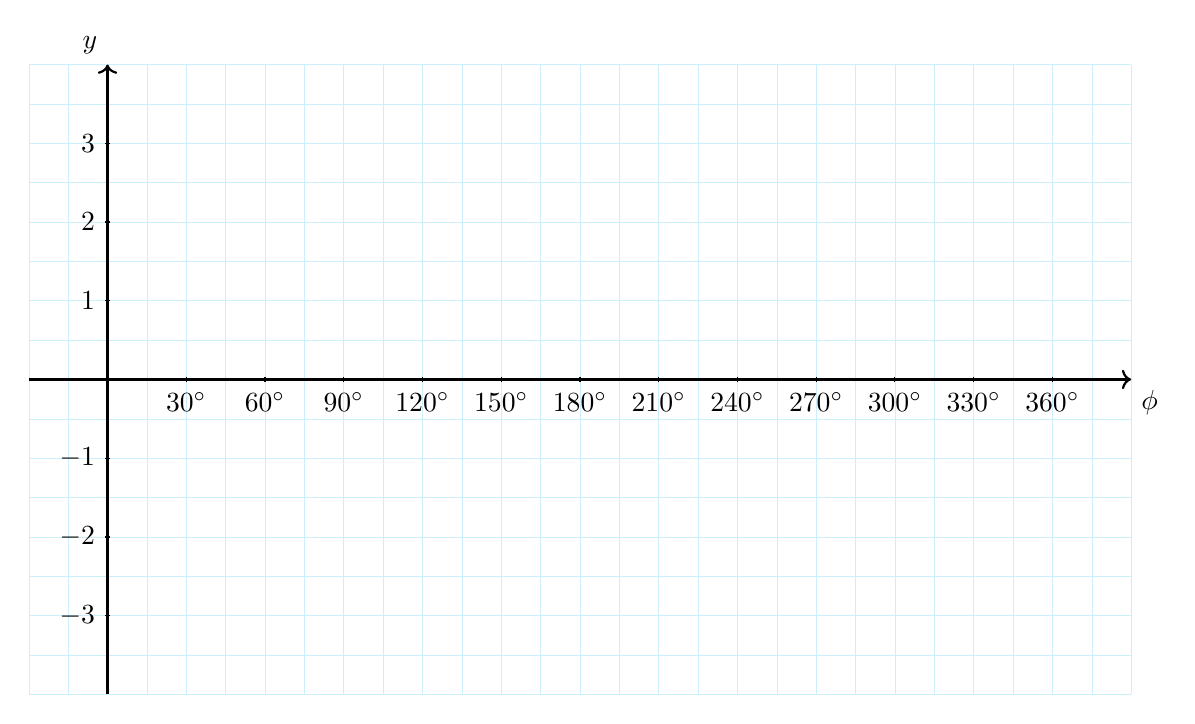
\begin{tikzpicture}
\draw[step = 0.5 cm, cyan!20 , very thin] (-1, -4) grid ( 13, 4);
\draw[thick, ->] (-1,0) -- (13,0) node[anchor = north west] {$\phi$};
\draw[thick, ->] (0,-4) -- (0,4) node[anchor = south east] {$y$};

\foreach \x [evaluate=\x as \degree using int(\x*30)] in {1,...,12}{ 
   \draw (\x cm, 1pt) -- (\x cm, -1pt) node[anchor = north] {$\degree^\circ$};
   }
\foreach \y in {-3,-2,-1,1,2,3}
   \draw (1pt, \y cm) -- (-1pt, \y cm) node[anchor = east] {$\y$};
\end{tikzpicture}}%% END Definition

\newcommand{\trigsysB}{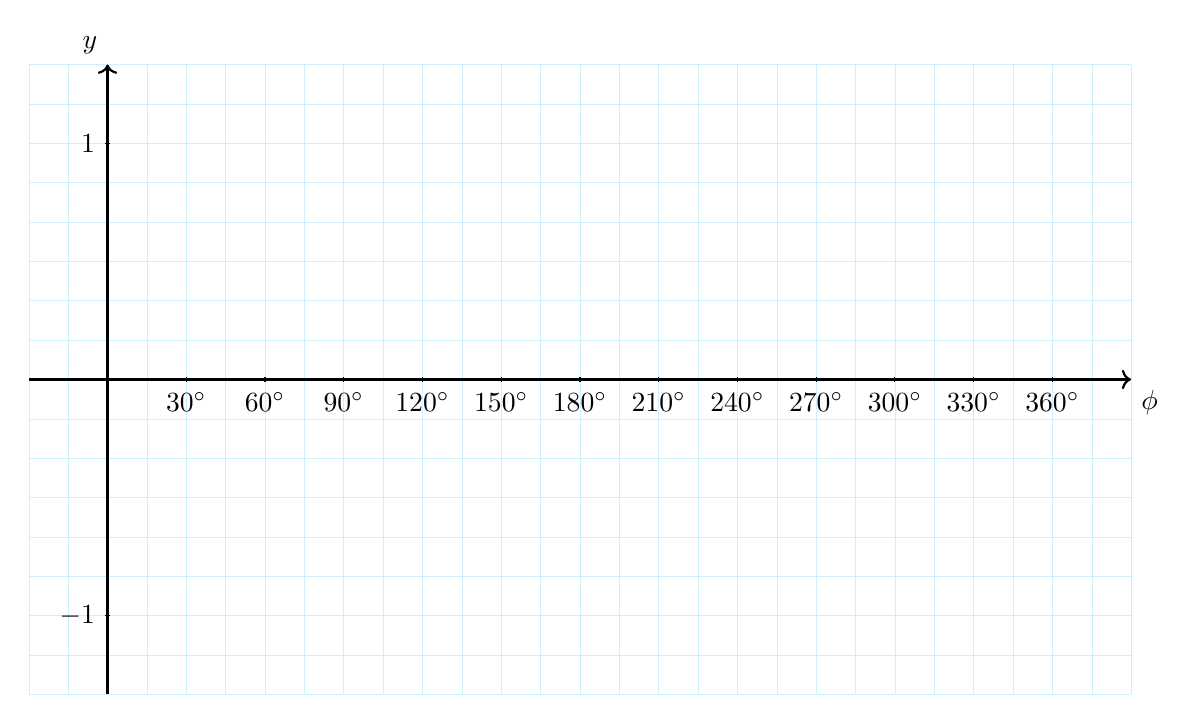
\begin{tikzpicture}\draw[step = 0.5 cm, cyan!20 , very thin] (-1, -4) grid ( 13, 4);
\draw[thick, ->] (-1,0) -- (13,0) node[anchor = north west] {$\phi$};
\draw[thick, ->] (0,-4) -- (0,4) node[anchor = south east] {$y$};

\foreach \x [evaluate=\x as \degree using int(\x*30)] in {1,...,12}{ 
   \draw (\x cm, 1pt) -- (\x cm, -1pt) node[anchor = north] {$\degree^\circ$};
   }
\foreach \y in {-1,1}
   \draw (1pt, \y *3cm) -- (-1pt, \y *3cm) node[anchor = east] {$\y$};

\end{tikzpicture}}%% END Definition

\newcommand{\trigsysC}{
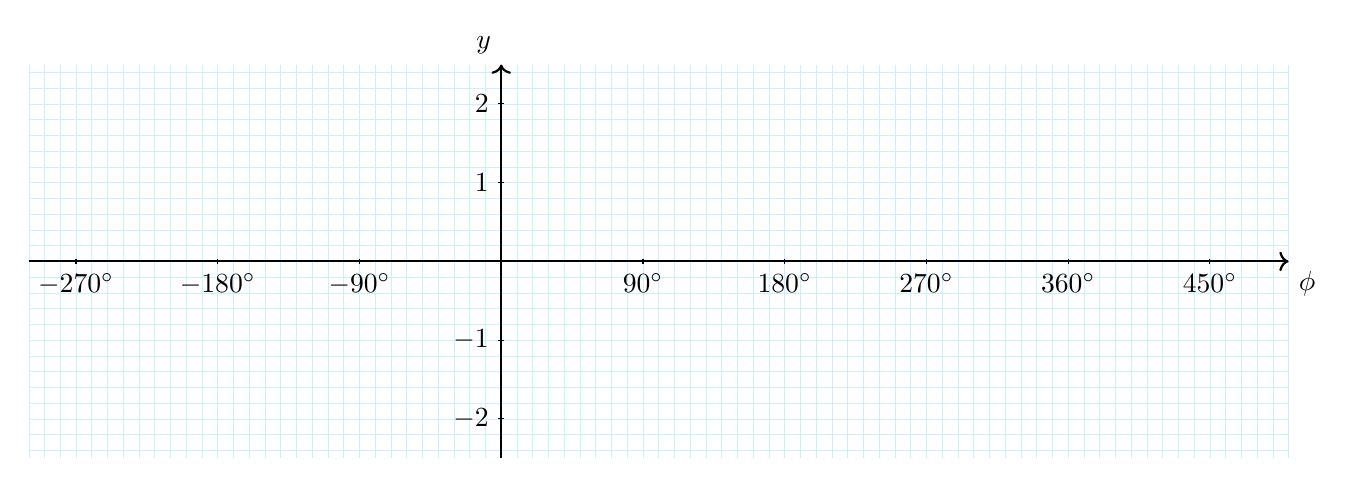
\begin{tikzpicture}
\draw[step = 0.2 cm, very thin, cyan!20] (-6, -2.5) grid ( 10, 2.5);
\draw[thick, ->] (-6,0) -- (10,0) node[anchor = north west] {$\phi$};
\draw[thick, ->] (0,-2.5) -- (0,2.5) node[anchor = south east] {$y$};

\foreach \x [evaluate=\x as \degree using int(\x*90)] in {-3,-2,-1,1,2,3,4,5}{ 
   \draw (\x *18mm, 1pt) -- (\x * 18mm, -1pt) node[anchor = north] {$\degree^\circ$};
   }
   
\foreach \y in {-2,-1,1,2}
   \draw (1pt, \y cm) -- (-1pt, \y cm) node[anchor = east] {$\y$};
\end{tikzpicture}}%% END Definition

\newcommand{\trigsysD}{
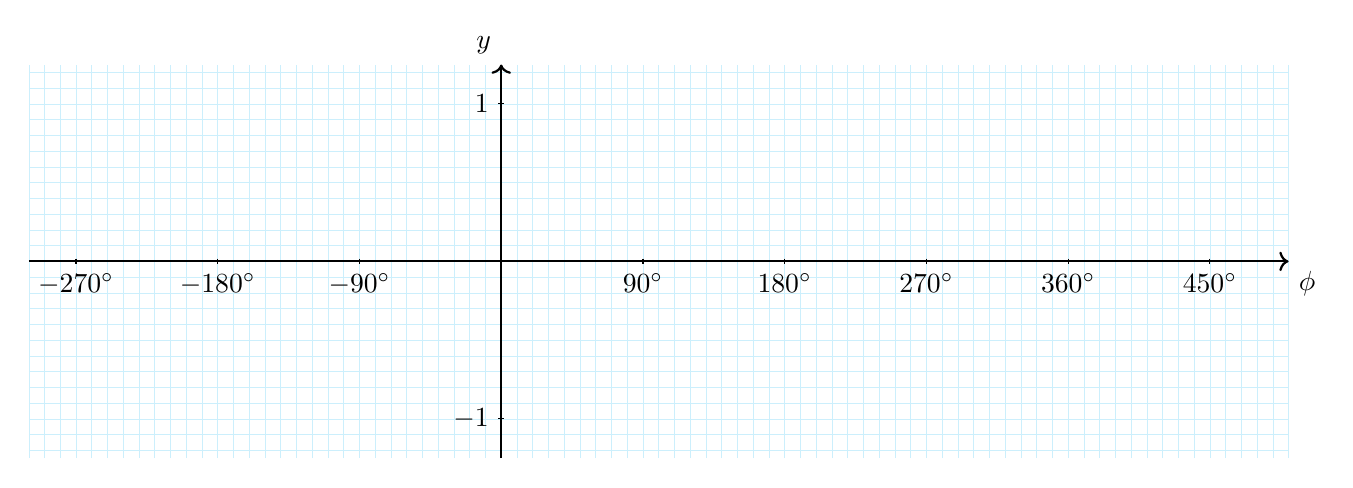
\begin{tikzpicture}
\draw[step = 0.2 cm, very thin, cyan!20] (-6, -2.5) grid ( 10, 2.5);
\draw[thick, ->] (-6,0) -- (10,0) node[anchor = north west] {$\phi$};
\draw[thick, ->] (0,-2.5) -- (0,2.5) node[anchor = south east] {$y$};

\foreach \x [evaluate=\x as \degree using int(\x*90)] in {-3,-2,-1,1,2,3,4,5}{ 
   \draw (\x *18mm, 1pt) -- (\x * 18mm, -1pt) node[anchor = north] {$\degree^\circ$};
   }
   
\foreach \y in {-1,1}
   \draw (1pt, \y *2cm) -- (-1pt, \y *2cm) node[anchor = east] {$\y$};
\end{tikzpicture}}%% END Definition


\newcommand{\trigsysDsin}{
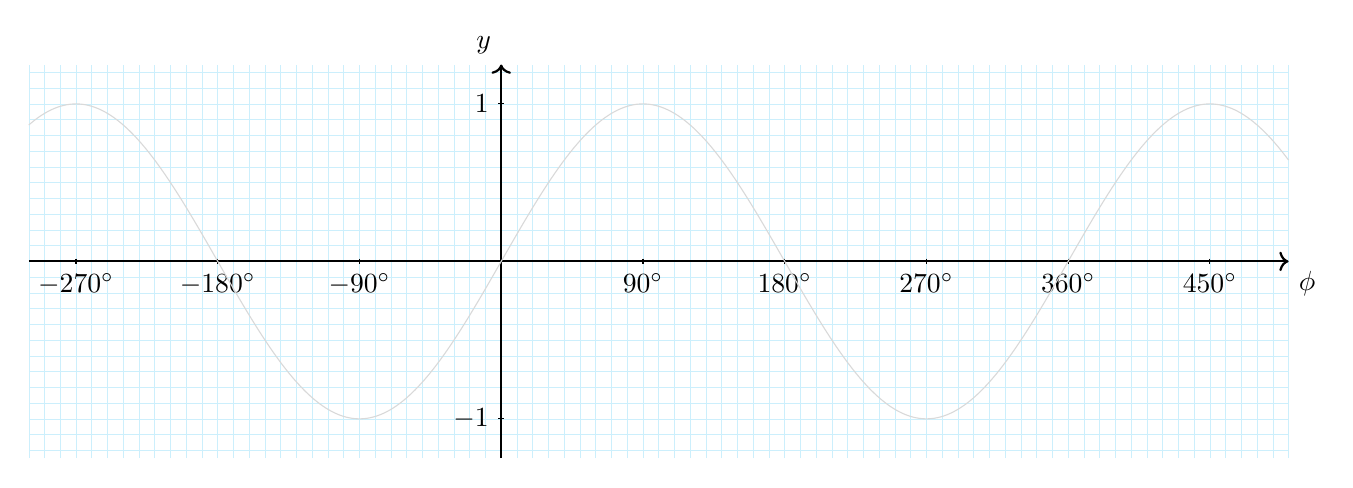
\begin{tikzpicture}
\draw[step = 0.2 cm, very thin, cyan!20] (-6, -2.5) grid ( 10, 2.5);
\draw[thick, ->] (-6,0) -- (10,0) node[anchor = north west] {$\phi$};
\draw[thick, ->] (0,-2.5) -- (0,2.5) node[anchor = south east] {$y$};

\foreach \x [evaluate=\x as \degree using int(\x*90)] in {-3,-2,-1,1,2,3,4,5}{ 
   \draw (\x *18mm, 1pt) -- (\x * 18mm, -1pt) node[anchor = north] {$\degree^\circ$};
   }
   
\foreach \y in {-1,1}
   \draw (1pt, \y *2cm) -- (-1pt, \y *2cm) node[anchor = east] {$\y$};

\draw[domain=-6:10,smooth,samples=200,variable=\x,gray!30] plot ({\x},{2*sin(\x*50)});
\end{tikzpicture}}%% END Definition

\newcommand{\trigsysDcos}{
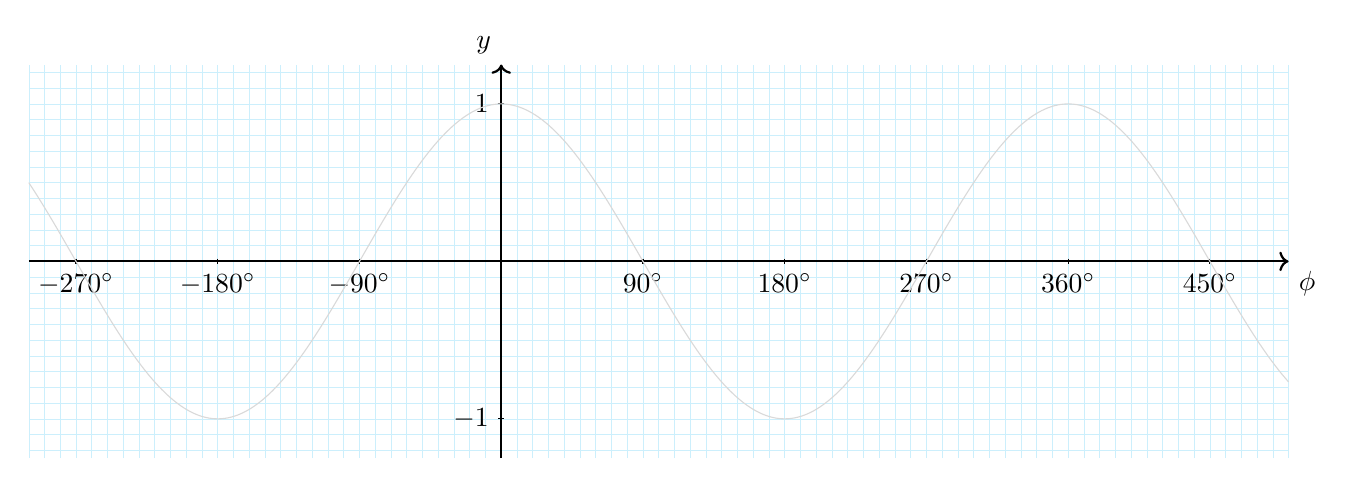
\begin{tikzpicture}
\draw[step = 0.2 cm, very thin, cyan!20] (-6, -2.5) grid ( 10, 2.5);
\draw[thick, ->] (-6,0) -- (10,0) node[anchor = north west] {$\phi$};
\draw[thick, ->] (0,-2.5) -- (0,2.5) node[anchor = south east] {$y$};

\foreach \x [evaluate=\x as \degree using int(\x*90)] in {-3,-2,-1,1,2,3,4,5}{ 
   \draw (\x *18mm, 1pt) -- (\x * 18mm, -1pt) node[anchor = north] {$\degree^\circ$};
   }
   
\foreach \y in {-1,1}
   \draw (1pt, \y *2cm) -- (-1pt, \y *2cm) node[anchor = east] {$\y$};

\draw[domain=-6:10,smooth,samples=200,variable=\x,gray!30] plot ({\x},{2*cos(\x*50)});
\end{tikzpicture}}%% END Definition


%%

\usepackage{bbwLayoutPageSty}


%%%%%%%%%%%%%%%  H E A D E R   &   F O O T E R %%%%%%%%%%%%%%%%%%%%
%% Headers
\fancyhf[HL]{\makebox{\includegraphics[width=30mm]{logos/bbw.pdf}}}%%
\fancyhf[HC]{\metaHeaderLine{}}%%
\fancyhf[FR]{\tiny{\shortAuthor{} (\today{})}}%%

\newcommand{\arbeitsblattHeader}{%%
  \begin{center}%%
    {\Large \fontfamily{qhv}\selectfont \arbeitsblattTitel{}}%%
\end{center}}%%


%%%%%%%%%%%%%%%%%%%%%%%%%%%%%%%%%%%%%%%%%%%%%%%%%%%%%%%%%%%%%%%%%%

\usepackage{amssymb} %% für \blacktriangleright
\renewcommand{\metaHeaderLine}{Arbeitsblatt}
\renewcommand{\arbeitsblattTitel}{Vektorgeometrie in $\mathbb{R}^3$}

\begin{document}%%
\arbeitsblattHeader{}

\newcounter{aufgabennummer}
\setcounter{aufgabennummer}{1}


\newcommand\aufgabeML[2]{
\textbf{Aufgabe \arabic{aufgabennummer}}:\,\,\\
#1  #2

\abplz{4}

\hrule

\stepcounter{aufgabennummer}
}




\renewcommand\aufgabeML[2]{\begin{samepage}%%
\textbf{Aufgabe \arabic{aufgabennummer}:}\,\,\\
#1%%\\  \TRAINER{#2}
%%
\TRAINER{#2}%%abplz{5.2}
\noTRAINER{\mmPapierBisEndeSeite}
%%\end{samepage}
\stepcounter{aufgabennummer}%%
\end{samepage}%%
}%%



\section{Vektorgeometrie in $\mathbb{R}^3$}
\subsection{Komponenten}

\aufgabeML{Welcher Vektor $\vec{s}$ beschreibt die Verschiebung, welche
den Punkt $A$ auf $A'$ abbildet?

$A = (6  | 9 | -1.5)$

$A' = (8 | 5 | 3.5)$

\vspace{22mm}
}{

Lösung: $\vec{s}$ = \LoesungsRaum{$\Spvek{2;-4;5}$}%%
}


\aufgabeML{Gegeben sind die folgenden Vektoren:
$$\vec{a} = \Spvek{1;2;x}; \vec{b} = \Spvek{x;y;-1} \text{ und } \vec{c} = \Spvek{z; 2z; 0} $$

Berechnen Sie $x$, $y$ und $z$ so, dass $\vec{a} + \vec{b} + \vec{c} =
0$.
}{%%

Lösung: \noTRAINER{\vspace{15mm}}\TRAINER{1. Aus der dritten
Komponente folgt $x=1$. Nun folgt aus der ersten Komponente, dass
$z=-2$ ; danach kann das $y$ aus der zweiten Komponente errechnet
werden: $y=2$}}
\newpage
\aufgabeML{Bestimmen Sie die fehlenden Parameter, damit gilt $\vec{a} = 3\cdot{}\vec{b}$

$$\vec{a} = \Spvek{6; -t; m} \text{ und } \vec{b}= \Spvek{-\frac{s}{4}; 3(t-1); 6.8m}$$
}{

Lösung:

\TRAINER{Komponentenweise
$s=-24$, $t=\frac34$, $m=0$}%% end TRAINER
}%% end AufgabeML



\newpage
\subsection{Längenprobleme}
\aufgabeML{
a) Bestimmen Sie den Betrag des Vektors $\vec{a}$:
$$\vec{b}=\Spvek{2;6;9}$$

b) Berechnen Sie:

$$\left|\Spvek{4;4;7}\right|$$


c) Bestimmen Sie mit dem Taschenrechner den Betrag des Vektors $\vec{c}$:
$$\vec{c}=\Spvek{3.5;-6;0}$$

%%\vspace{22mm}
}{
a) $|\vec{a}| = \LoesungsRaum{11}$

b) $|\vec{b}| = \LoesungsRaum{9}$

c) $|\vec{c}| \approx \LoesungsRaum{6.94622199472}$
}
\newpage

\aufgabeML{%%
a) Der Vektor $\vec{v}$ habe die Struktur $\Spvek{3;v_y;2}$. Es gilt
$|\vec{v}| = 7$. Berechnen Sie $v_y$.

b) 
Der Vektor $\vec{v}$ habe folgende Struktur:
$$\vec{v}=\Spvek{a;6;a+3}$$
Wir wissen, dass $$|\vec{v}|=\sqrt{125}$$
Berechnen Sie $a$. (Tipp: Zweiklammeransatz)
}{

Lösung: a)
\TNT{4}{
$$\sqrt{2^2 + 3^2 + v_y^2}=7$$
$$13 + v_y^2=49$$
$$v_y^2=36$$
$$L_{v_y} = \{-6; 6\}$$
}%% end TNT 4

Lösung b)
$\TRAINER{a=-8 \text{ oder } 5}$\\
\TRAINER{Es gilt
$$\sqrt{125} = \sqrt{a^2 + 6^2 + (a+3)^2}$$
Somit
$$125 = a^2 + 36 + a^2 + 6a + 9$$
Grundform:
$$a^2 + 3a -40 = 0$$
Zweiklammeransatz:
$$(a+8)(a-5) = 0$$
Somit $L_a = \{-8, 5\}$}
}

\newpage


\aufgabeML{Gegeben sind die Punkte:
$$A= (7 | 5.5 | -3) \text{ und } B=(5|-2|0)$$

Berechnen Sie die folgenden Terme:

\vspace{22mm}
}{$$\overrightarrow{OA}
=\LoesungsRaum{\Spvek{7;5.5;-3}}$$
$$\overline{AB} \approx \LoesungsRaum{8.3217}$$}


\aufgabeML{Gegeben sind die Punkte $A=(5|1)$ und $B=(8|5)$.

a) Bestimmen Sie die Vektoren $\overrightarrow{OA}$,
$\overrightarrow{AB}$

b) Geben Sie die Länge des Vektors $\overrightarrow{BA}$ an.

}{

Lösung zu a) $$\overrightarrow{OA} = \LoesungsRaum{\Spvek{5;1}}$$

$$\overrightarrow{AB} = \LoesungsRaumLen{50mm}{\overrightarrow{OB} - \overrightarrow{OA}
=  \Spvek{8;5} - \Spvek{5;1} = \Spvek{3;4}}$$

Lösung zu b)

$$|\overrightarrow{AB}| = \LoesungsRaumLang{\sqrt{3^2+4^2} = \sqrt{25}= 5}$$
}%% end aufgabeML
\newpage

\aufgabeML{Bestimmen Sie alle Punkte der $xy$-Ebene, welche von den
beiden Punkten $A=(7|6)$ und $B=(-1|2)$ den selben Abstand haben.}{
Lösung:

$$\LoesungsRaumLang{y = -2x + 10}$$

\TRAINER{
Wir definieren $P := (x|y)$. Nun gelte $|\overrightarrow{AP}| =
|\overrightarrow{BP}|$. Mit den Zahlen:

$$\bigg|\Spvek{7-x;6-y}\bigg| = \bigg|\Spvek{-1-x;2-y}\bigg|$$
Wenn wir nun den Abstand rechnen, so erhalten wir:

$$\sqrt{(7-x)^2 + (6-y)^2} = \sqrt{(-1-x)^2 + (2-y)^2}$$
Beidseitig quadrieren und ausmultiplizieren:
$$49-14x+x^2 + 36-12y+y^2  =  1 + 2x + x^2  + 4 - 4y + y^2$$
Quadrate beidseitig subtrahieren und zusammenfassen:
$$49+36-1-4 = 8y + 16 x$$
Grundform:
$$y= -2x + 10$$
Alle Punkte auf der Geraden $-2x+10$ sind von $A$ und $B$ gleich weit entfernt.

}%% end TRAINER

}%% end aufgabeML





\aufgabeML{%%
Berechnen Sie den Umfang des Dreiecks
$$A=(7|2|6), B=(-4|3|-1), C=(0;0;8)$$
}{
Umfang $\approx \LoesungsRaumLang{30.9222}$

\TRAINER{
$$\overrightarrow{AB} = \Spvek{7-(-4);2-3;6-(-1)} = \Spvek{11;-1;7}$$
$$\overrightarrow{BC} = \Spvek{-4-0; 3-0; -1-8} = \Spvek{-4;3;-9}$$
$$\overrightarrow{AC} = \Spvek{7-0;2-0;6-8} = \Spvek{7;2;-2}$$
}%% end TRAINER

}%% end aufgabeML
\newpage


\aufgabeML{Bestimmen Sie die Länge der Seitenhalbierenden $s_a$ im
Dreieck $\Delta ABC$\\
(es gelte $e_x=e_y=e_z=1$):

$$A=(1|1|2); B=(3|4|5); C=(2|9|6)$$

}{Lösung: Die Länge misst \LoesungsRaumLang{ca. $6.6895$} (Einheiten)
\TRAINER{
Erstens den Mittelpunkt $M_a$ der Strecke $\overline{BC}$ rechnen:
$$M_a = (2.5| 6.5 | 5.5)$$
Nun den Vektor $\vec{s_a} = \overrightarrow{AM_a}$ bestimmen:
$$\vec{s_a} = \Spvek{2.5-1; 6.5-1; 5.5-2} = \Spvek{1.5; 5.5; 3.5}$$
TR: Dreidimensionaler Pythagoras:
$$|s_a| = \sqrt{1.5^2 + 5.5^2 + 3.5^2} \approx 6.6859$$
}%% end TRAINER
}%% end aufgabeML
\newpage
\aufgabeML{Berechnen Sie alle Punkte auf der $y$-Achse, welche vom
Punkt $P=(2|-3|4)$ fünf Einheiten entfernt sind.}{

Lösung:
\TRAINER{Ansatz Punkt = $\Spvek{0;y;0}$ Dann gilt

$$5 = \sqrt{(2-0)^2 + (-3-y)^2 + (4-0)^2}$$

$y=-3\pm \sqrt{8} \approx -5.83 \text{ bzw. } -0.172$}
}
\newpage
\aufgabeML{Bestimmen Sie mit dem Taschenrechner alle möglichen Punkte
auf der $x$-Achse, welche vom Punkt $A=(-4|3|12)$ die dreifache Entfernung wie
vom Punkt $B=(16|2|-1)$ haben.}{
Lösung: $\LoesungsRaumLang{}$
\TRAINER{Ansatz: Gesuchter Punkt $P$ hat Koordinaten $(x|0|0)$.

Dann gilt

$\overline{AP} = 3\cdot{} \overline{BP}$

TR: solver: $$\lx = \{10.15; 26.85\}$$
}%% end TRANIER
}%% end aufgabeML
\newpage

\aufgabeML{Gegeben sind die Drei Punkte $A=(1|2|-3)$, $B=(6|-2|4)$ und
$C=(2|3|-5)$.

Welcher Punkt in der $xz$-Ebene ist von all den drei Punkten gleich
weit entfernt?
}{Lösung \LoesungsRaumLang{$P=\Spvek{\frac{126}{17};0;\frac{-39}{17}}$}
}%% end aufgabe ML
\newpage

\subsection{Vielfaches im Raum}

\aufgabeML{Berechnen Sie $\vec{b}$ so, dass $\vec{b}$ den Betrag 5 hat
und dem Vektor $\vec{a}$ entgegengesetzt ist:
$$\vec{a} = \Spvek{4;0;-3}$$

\vspace{12mm}
}{$$\vec{b} = \LoesungsRaum{\Spvek{-0.8;0;0.6}}$$}
\newpage


\aufgabeML{
Gegeben sind die drei Vektoren $\vec{a}=\Spvek{1;2;0}$,
$\vec{b}=\Spvek{-4;-3;5}$ und
$\vec{c}=\Spvek{2;-3;1}$.

Berechnen Sie den Vektor $\vec{d}$, wenn gilt:

$$ -\vec{a} + 5\left( \vec{d}-\frac13\vec{b} \right) = 2\vec{c}$$

}{Der Lösungsvektor $\vec{d}$ ist gleich
\TRAINER{$\Spvek{-\frac13;-\frac95;\frac{31}{15}}$}

Kontrollieren Sie Ihr Ergebnis mit dem Taschenrechner.
}



\aufgabeML{Berechnen Sie den Vektor $\vec{v} = \vec{a}+2.5\vec{b}
-3\vec{c}$ mit:

$$\vec{a}= \Spvek{4;3;-1}; \vec{b}= \Spvek{1;-1;0} \vec{c}= \Spvek{-2;-1;1}$$}%%
{Lösung: \noTRAINER{\vspace{22mm}}\TRAINER{$$\vec{v} = \Spvek{4 + 2.5\cdot{}1 - 3\cdot{}(-2);3 +
2.5\cdot{}(-1) -3\cdot{}(-1);-1 +0 -3\cdot{}1}= \Spvek{12.5;3.5;-4}$$}}%%

\newpage

\aufgabeML{Kollinear:

Bestimmen Sie $x$ und $y$ so, dass $\vec{a}$ kollinear zu $\vec{b}$
ist:

$$\vec{a} = \Spvek{2;3;x}; \vec{b} = \Spvek{-x;5;y}$$
}{$x=\LoesungsRaum{\frac{-10}3}$ und $y = \LoesungsRaum{\frac{-50}9}$

\TRAINER{Es gilt $\vec{a} = \lambda\cdot{}\vec{b}$.
Aus der 2. Komponente folgt $3 = \lambda\cdot{}5$ und somit $\lambda =
\frac35$.\\

Dieses $\lambda$ setzen wir in die erste Komponente einund
erhalten $$2 = \frac35 \cdot{-x}$$
ergo $$x = \frac{-10}3$$

Nun können wir aus der 3. Komponente das $y$ berechnen:
$$x = \lambda\cdot{}y$$
$x$ und $\lambda$ einsetzen:
$$\frac{-10}3 = \frac35 \cdot{} y$$
und somit
$$y = \frac{-50}9$$}%% end TRAINER
}%% end aufgabeML

\aufgabeML{Gegeben seien die Vektoren $\vec{a}$, $\vec{b}$ und
$\vec{c}$.

Des weiteren ist die folgende Beziehung bekannt:

$$2\vec{c}-\frac14 \vec{b} - 2(\vec{a}+\vec{d})= 3(\vec{a}+\vec{b}+\vec{d})$$

Geben Sie den Vektor $\vec{d}$ als Linearkombination der Vektoren
$\vec{a}$, $\vec{b}$ und $\vec{c}$ an:
}{$$\vec{d}  = \LoesungsRaumLang{-5\vec{a} -\frac{13}4 \vec{b} + 2\vec{c}}$$}
\newpage

\aufgabeML{Bestimmen Sie die fehlenden Koordinaten, wenn beide der
folgenden Eigenschaften zutreffen sollten:

a) 
$$\vec{s} = \vec{a} + 2\vec{b} -5 \vec{c}$$
\textbf{und} b)\\
$$\vec{a} \text{ ist kollinear zu } \vec{c}$$
Für
$$\vec{a}=\Spvek{3;-2}; \vec{b} = \Spvek{b_x; b_y}; \vec{c}
= \Spvek{-2;c_y}; \vec{s} = \Spvek{5;5}$$}%%
{$b_x = \LoesungsRaum{-4}$, $c_y = \LoesungsRaum{\frac43}$ und $b_y
= \LoesungsRaum{\frac{41}6}$
\TRAINER{
Aus a) folgt:
\gleichungZZ{3+2b_x -5\cdot{}(-2)}{5}{-2+2\cdot{}b_y -5\cdot{}c_y}{5}
Aus der oberen Gleichung folgt:
$$2b_x + 10 = 2$$
und somit
$$b_x=-4$$
Weil $\vec{a}$ kollinear zu $\vec{b}$ folgt aus der 1. Komponente:
$$\vec{a} = \lambda\cdot{}\vec{b} \Longrightarrow 3 = \lambda \cdot{}
(-2) \Longrightarrow \lambda = \frac{-3}2$$
Wegen $-2 = \lambda \cdot{} c_y$ folgt, dass $c_y = \frac43$.
Dies können wir in die 2. Gleichung einsetzen:
$$2b_y -5\cdot{}\frac43 = 7$$
und somit
$$b_y = \frac{41}6$$
}%% end TRAINER
}%% end aufgabeML

\aufgabeML{%
Einheitsvektor:

Gegeben ist der Vektor $\vec{a}$:
$$\vec{a} = \Spvek{\sqrt{7};-2;3.8}$$

Skalieren Sie den Vektor $\vec{a}$ mit einem Skalar $s$ so, dass er die Länge 1 hat.


}{%
Lösung: $s=\LoesungsRaum{\frac{5\cdot{}\sqrt{159}}{318} \approx 0.1983}$
}
\newpage
\aufgabeML{Bestimmen Sie den Parameter $p$ so, dass es sich beim
folgenden um einen Einheitsvektor handelt:
$$\Spvek{0.7; k; \frac1{10}}$$
(Mit Taschenrechner auf 3 signifikante Stellen angeben.)


}{Lösung = \LoesungsRaumLang{$\sqrt{2}/2 \approx 0.707$}}

\newpage

\aufgabeML{
Berechnen Sie alle Punkte $A$ auf der Geraden $PQ$, die sieben Einheiten
von $P$ entfernt sind.

Gegeben: $$P=(3|9|1); Q=(6|8|-4)$$
}{Lösung \TRAINER{mit Einheitsvektor:

$$\Spvek{3;9;1} \pm \frac{\sqrt{35}}{5}\cdot{}\Spvek{3;-1;-5}$$

}%% end TRAINER
}%% end AufgabeML



\newpage
\subsection{Linearkombination}
\aufgabeML{Stellen Sie den Vektor $\vec{z}$ als Linearkombination von
$\vec{a}$, $\vec{b}$ und $\vec{c}$ dar.
$$\vec{a} = \Spvek{4;2;-7};
  \vec{b} = \Spvek{1;-4;-5};
  \vec{c} = \Spvek{4;0;-3};
  \vec{z} = \Spvek{48;48;84}$$

\vspace{12mm}
}{$$\vec{z} = \LoesungsRaum{42}\cdot{}\vec{a}
+ \LoesungsRaum{9}\cdot{}\vec{b} + \LoesungsRaum{-129}\cdot{}\vec{c}$$}
\newpage


\aufgabeML{Lässt sich der Vektor $\vec{a}$ als Linearkombination von
$\vec{u}$, $\vec{v}$ und $\vec{w}$ schreiben? Falls ja, geben Sie die
Linearkombination explizit an, falls nein, begründen Sie warum nicht.
$$\vec{a} = \Spvek{5;6;-7}$$

a) $$\vec{u} = \Spvek{1;0;1}; \vec{v} = \Spvek{0;1;1}; \vec{w} = \Spvek{1;1;0}$$

b) $$\vec{u} = \Spvek{1;0;0}; \vec{v} = \Spvek{1;0;1}; \vec{w} = \Spvek{0;0;1}$$

c) $$\vec{u} = \Spvek{1;0;0}; \vec{v} = \Spvek{1;1;0}; \vec{w} = \Spvek{1;1;1}$$
}{
Lösung zu a):\\
\noTRAINER{\vspace{30mm}}
\TRAINER{\gleichungDD{\alpha+\gamma}{5}{\beta+\gamma}{6}{\alpha+\beta}{-7}
$$\Longrightarrow \alpha = 5-\gamma; \beta = 6-\gamma$$
$$\alpha + \beta = -7 \Longrightarrow
5-\gamma+6-\gamma=-7 \Longrightarrow \gamma = 9$$
$$\Longrightarrow  \beta = -3; \alpha = -4$$
$$-4\vec{u} -3\vec{v} +9\vec{w} = \Spvek{5;6;-7}$$
}%% end TRAINER

Lösung zu b):\\
\noTRAINER{\vspace{30mm}}
\TRAINER{
Dies ist nicht lösbar, denn zum einen sind $\vec{u}$, $\vec{v}$ und
$\vec{w}$ nicht linear unabhängig und zum anderen kann die zweite
Komponente (die $y$-Koordinate) gar nicht 6 werden, denn die
$y$-Koordinate ist in allen drei gegebenen Vektoren = 0.\\
}%% end TRAINER

Lösung zu c):\\
\noTRAINER{\vspace{30mm}}
\TRAINER{
Beginne mit der $z$-Koordinate $\Longrightarrow \gamma=-7$. Verfahre
von unten her weiter mit der $y$-Koordinate...

$$-\Spvek{1;0;0} +13\Spvek{1;1;0}-7\Spvek{1;1;1} = \Spvek{5;6;-7}$$
}%% end TRAINER
}%% end aufgabeML
\newpage





\aufgabeML{Gegeben sind die Vektoren
$$\vec{a}= \Spvek{-5;3;-7},
 \vec{b} = \Spvek{-3;-3;2} \text{ und }
 \vec{c} = \Spvek{0;2;-2}$$


Berechnen Sie $\vec{d}$ so, dass
$\vec{a}+\vec{b}+\vec{c}+\vec{d}=\vec{0}$ ergibt.
\vspace{22mm}
}{$\vec{d} = \LoesungsRaum{\Spvek{8;-2;7}}$}

\subsection{lineare Abhängigkeit}


\aufgabeML{Sind die beiden folgenden Vektoren voneinander linear
abhängig?

$\vec{a} = \Spvek{2;12;7}$, $\vec{b} = \Spvek{-3;-18;10}$

}{Die beiden Vektoren sind linear \LoesungsRaumLang{unabhängig}.}

\newpage


\aufgabeML{Für welches $z$ sind die drei folgenden Vektoren
voneinander linear abhängig?

$\vec{a} = \Spvek{1;-1;3}$,
$\vec{b} = \Spvek{4;5;1}$
$\vec{c} = \Spvek{2;-4;z}$
}{
Lösung $z = \LoesungsRaum{\frac{76}9}$\TRAINER{, denn damit geht die
Gleichung $$s\cdot{}\vec{a} + t\cdot{}\vec{b} = \vec{c}$$ auf und
somit ist $\vec{c}$ eine Linearkombination von $\vec{a}$ und $\vec{b}$}.
}


\aufgabeML{%% Frommenwilere Geometrie Aufga 51 S. 189
Welche Vektoren sind voneinander linear abhängig?

$$\vec{p} = \Spvek{3;7}; \vec{q} = \Spvek{5;9} ; \vec{r} = \Spvek{4.5;10.5}$$
}{Lösung: \LoesungsRaumLang{$\vec{p}$ und $\vec{r}$, denn $\vec{r} = 1.5\cdot{}\vec{p}$}}

\aufgabeML{%% Frommenwilere Geometrie Aufga 51 S. 189
Welche Vektoren sind voneinander linear abhängig?

$$\vec{p} = \Spvek{1;4;3}; \vec{q} = \Spvek{-2;-8;6} ; \vec{r} = \Spvek{0.5;2;-1.5}$$
}{Lösung: \LoesungsRaumLang{$\vec{q}$ und $\vec{r}$, denn $\vec{q} = -4\cdot{}\vec{r}$}}




\end{document}
